\documentclass[11pt]{article}
\usepackage[T1]{fontenc}
\usepackage[utf8]{inputenc}
\usepackage{times}
\usepackage{inconsolata}
\usepackage{amsmath}
\usepackage{framed}
\usepackage{graphicx}
\usepackage{hyperref}
\hypersetup{colorlinks=true, linkcolor=blue, urlcolor=blue}
\usepackage{fancyvrb}
\usepackage[english]{babel}
\usepackage{enumitem}
\usepackage{float}
\usepackage{pdfpages}


% reqT tex notations
\usepackage{xcolor}
\definecolor{entityColor}{RGB}{0,100,200}
\definecolor{attributeColor}{RGB}{0,100,50}
\definecolor{relationColor}{RGB}{160,0,30}
\usepackage{listings}
\lstdefinestyle{reqT}{
  belowcaptionskip=1\baselineskip,
  breaklines=true,
  showstringspaces=false,
  basicstyle=\footnotesize\sffamily,
  emph={Ent,Meta,Item,Label,Section,Term,Actor,App,Component,Domain,Module,Product,Release,Resource,Risk,Service,Stakeholder,System,User,Class,Data,Input,Member,Output,Relationship,Design,Screen,MockUp,Function,Interface,State,Event,Epic,Feature,Goal,Idea,Issue,Req,Ticket,WorkPackage,Breakpoint,Barrier,Quality,Target,Scenario,Task,Test,Story,UseCase,VariationPoint,Variant},
  emphstyle=\bfseries\color{entityColor},
  emph={[3]Attr,Code,Constraints,Comment,Deprecated,Example,Expectation,FileName,Gist,Image,Spec,Text,Title,Why,Benefit,Capacity,Cost,Damage,Frequency,Min,Max,Order,Prio,Probability,Profit,Value,Status},
  emphstyle={[3]\color{attributeColor}},
}
\lstset{style=reqT}

% end





\setlist[itemize]{noitemsep}
\title{{\bf LAB 1:\\Requirements Modeling}\\ Preparations and instructions}
\author{Björn Regnell, Emil Hammarström}
\date{\today}
\begin{document}
\maketitle

\section{Introduction}

\subsection{Purpose}

This document provides instructions for getting acquainted with the reqT ecosystem and the modeling of requirements using \textit{Entities}, \textit{Attributes}, and \textit{Relations}.
In other words, the purpose of this lab is learning how to use reqT, and preparing the mental model of viewing requirements as a \href{https://en.wikipedia.org/wiki/Tree_(data_structure)}{tree structure}.
The preparations will help you learn how to navigate the reqT tools.
The first laboration part will deepen your understanding of requirements as a tree structure, and the second part will introduce the metamodel, and a more advanced usage of reqT.

\subsection{Background}

In this lab you will learn how to get started with requirements modeling through the open source tool
\href{http://reqT.org}{reqT.org}, and reflect on how you could model requirements in your own project.
The reqT tool enables scalable requirements modeling, ranging from small models of a couple of features to large
models containing elaborate structures of thousands of requirements.
Requirements engineering is a dynamic process where the understanding of an imagined future system
(of systems) is evolving over time.
During this evolution we can capture the knowledge and creative ideas that we elicit in various ways,
depending on how we foresee the (later) usage of that knowledge.
For example, we could create and use spreadsheets, post-it notes, emails, wikis, video clips,
mockups, sketches, diagrams, mathematical specifications, etc.
If we want to keep track of many different types of inter-related requirements and if we see a future benefit
of more structure beyond just a flat list, one option is to use requirements models where requirements-related
information is expressed using relevant \textit{Entity}, \textit{Attribute}, and \textit{Relation} concepts to capture
what we want to model, as illustrated by this lab and the metamodel of reqT seen in Figure~\ref{figure:metamodel}.

\begin{figure}[H]
  \centering
  \includegraphics[width=\textwidth]{metamodel-simple.pdf}
  \caption{Some classes in the reqT metamodel.}
  \label{figure:metamodel}
\end{figure}

\clearpage\newpage
\section{Preparations}\label{section:preparations}
Throughout the lab you will find framed command snippets. Commands prefixed with \textbf{reqT>} are issued in the reqT-REPL. The \textbf{\$} prefix denotes a command issued in a terminal and may sometimes be followed by some output.
\subsection{Installing and running reqT}\label{section:preparations:installation}

\subsubsection{Prerequisites}
\begin{framed}
\noindent Open/Oracle JDK8+ (Java Development Kit)
{\footnotesize\begin{verbatim}
    $ java -version
    openjdk version "1.8.0_144"
    OpenJDK Runtime Environment (build 1.8.0_144-b01)
    OpenJDK 64-Bit Server VM (build 25.144-b01, mixed mode)
\end{verbatim}}
\noindent or
{\footnotesize\begin{verbatim}
    $ java -version
    java version "1.8.0_144"
    Java(TM) SE Runtime Environment (build 1.8.0_144-b01)
    Java HotSpot(TM) 64-Bit Server VM (build 25.144-b01, mixed mode)
\end{verbatim}}
\noindent If your output is similar to this,
{\footnotesize\begin{verbatim}
    $ java -version
    zsh: command not found: java
\end{verbatim}}
\noindent you may refer to the material in the section \textit{Installera JDK} \href{http://cs.lth.se/pgk/verktyg/}{here}
\end{framed}

\subsubsection{Linux \& OS X}\label{section:preparations:installation:unix}
The reqT.zip contains the reqT-REPL and reqT-webeditor, preferred installation steps:

\begin{framed}
\noindent Visit \url{https://github.com/reqT/reqT-webapp/releases} and download the latest reqT.zip. Open up a terminal and change directory to where you placed the zip and extract it:
{\footnotesize\begin{verbatim}
    $ cd <reqT.zip path>
    $ unzip reqT.zip
    Archive:  reqT.zip
      creating: reqT/
      creating: reqT/server/
      ...
    $ ls
    reqT  reqT.zip
\end{verbatim}}
\noindent You will now see a folder named \texttt{reqT} which contains the reqT-REPL (\textit{reqT.jar}) and reqT-webeditor (\textit{start.sh} start script).
\end{framed}

\subsubsection{Windows 10}\label{section:preparations:installation:windows}

\begin{enumerate}
\item Visit \url{https://github.com/reqT/reqT-webapp/releases} and download the latest reqT.zip
\item Unzip it (using the Windows File Explorer)
\end{enumerate}

To start the webeditor double-click the \textit{start.bat} file -- Figure~\ref{figure:cmd-running-webapp} shows the webapp running in the CMD.


To start the REPL double-click the \textit{reqT.bat} file -- you should be greeted by a view similar to Figure~\ref{figure:reqt-repl}.

\begin{figure}[H]
  \centering
    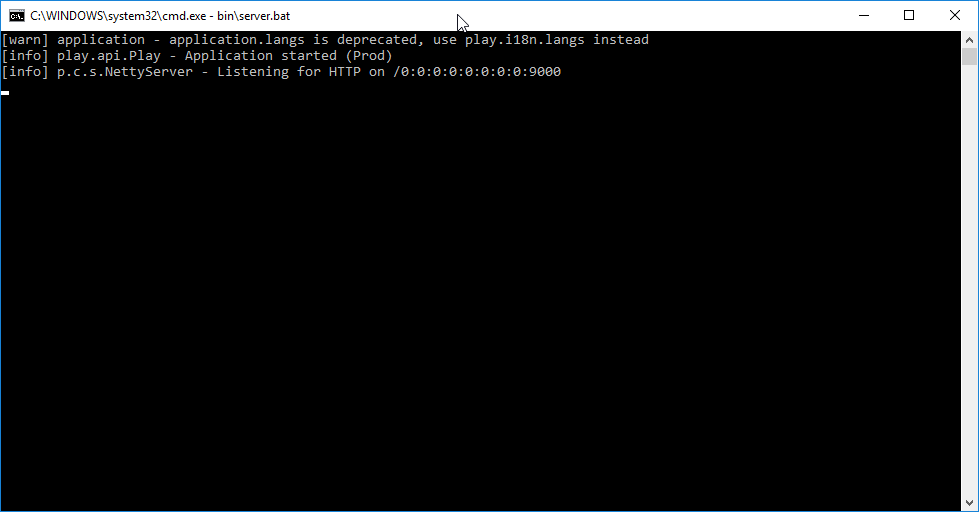
\includegraphics[width=\textwidth]{cmd_running_webapp.png}
  \caption{A Windows CMD running the webeditor}
  \label{figure:cmd-running-webapp}
\end{figure}

\subsubsection{reqT--REPL}

To enter the reqT REPL (\href{https://en.wikipedia.org/wiki/Read\%E2\%80\%93eval\%E2\%80\%93print\_loop}{Read-Eval-Print-Loop})
run \texttt{java -jar reqT.jar} --- you should be greeted with the output seen in Figure~\ref{figure:reqt-repl}.

\begin{figure}[H]
  \centering
    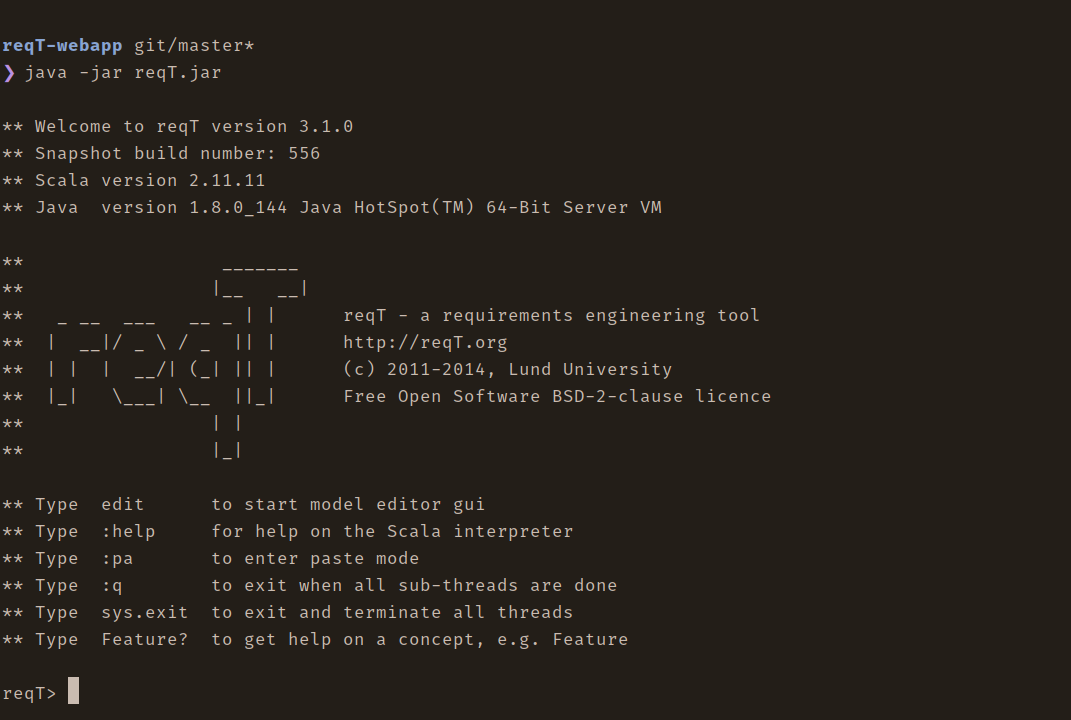
\includegraphics[width=\textwidth]{reqt-repl}
  \caption{reqT-REPL}
  \label{figure:reqt-repl}
\end{figure}

In the reqT console these keystrokes and commands work as follows:
{\footnotesize 
\begin{itemize}[label={}]
\item <Ctrl+A> to move the cursor to the beginning of a line.
\item <Ctrl+E> to move the cursor to the end of a line.
\item <Ctrl+K> ''kill'': clears text after the cursor.
\item <Arrow Left/Right> to move the cursor backward/forward within a line. 
\item <Arrow Up/Down> to move backward/forward in the command history. 
\item <TAB> to invoke code completion.
\item \verb+:q+ to quit reqT when all threads and windows have been exited.
\item \verb+:help+ to get help on console commands.
\item \verb+sys.exit+ to exit reqT and kill all threads and any windows without saving.
\end{itemize}
}

\begin{framed}
\noindent reqT wraps the scala REPL, enter:
{
  \footnotesize\begin{verbatim}
    reqT> println("Requirements, requirements, requirements!")
  \end{verbatim}
}
\noindent This also means that you have access to the JDK --- java libraries.
\noindent The command below will utilize your favorite GUI library to display a message dialog!
{
  \footnotesize\begin{verbatim}
    reqT> javax.swing.JOptionPane.showMessageDialog(null,"Hello Swing!")
  \end{verbatim}
}
\end{framed}

\subsubsection{reqT--webeditor}

\begin{framed}
\noindent To start the reqT-webeditor run the start script in the reqT folder with the terminal command (Windows users may refer to Section~\ref{section:preparations:installation:windows}):
{
  \footnotesize\begin{verbatim}
    $ ./start.sh
    [info] play.api.Play - Application started (Prod)
    [info] p.c.s.NettyServer - Listening for HTTP on /0:0:0:0:0:0:0:0:9000
  \end{verbatim}
}

\noindent Once started visit the url \url{localhost:9000} using \textit{Google Chrome} --- you should now be greeted by the page seen in Figure~\ref{figure:webeditor-expected}.
\end{framed}

\textit{Note:} the webeditor is currently only supported on Google Chrome

\begin{figure}[H]
  \centering
    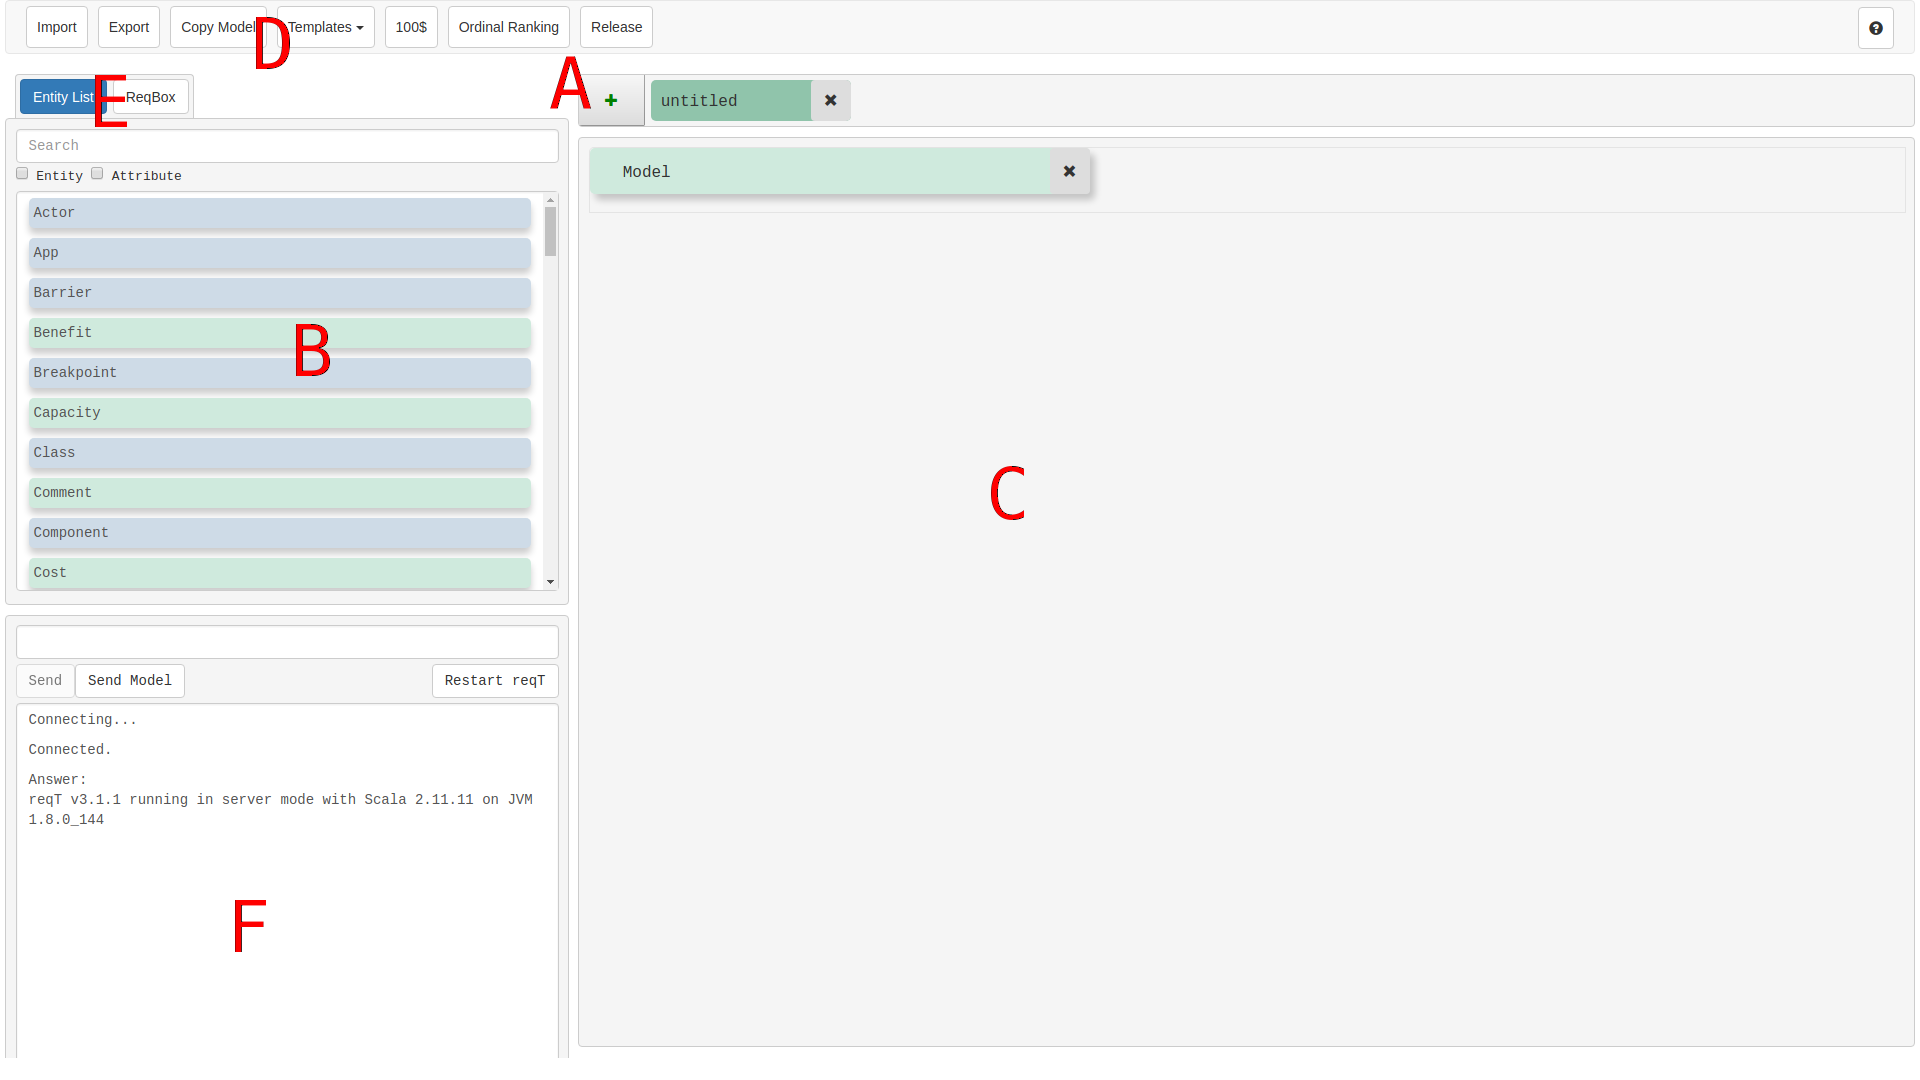
\includegraphics[width=\textwidth]{reqt-webeditor-entitylist-state-annotated.png}
  \caption{reqT-webeditor with component annotations}
  \label{figure:webeditor-expected}
\end{figure}

The reqT-webeditor allows the use of common shortcuts such as \texttt{CTRL-C, CTRL-V, DEL}. The symbols $A-F$ describe general parts of the application:

\begin{itemize}
\item $A$ - Add-button used to create new models, followed by model tabs (right of the add-button).
\item $B$ - Entity \& attribute list, from which you may drag and drop objects into view $C$
\item $C$ - Model tree view
\item $D$ - Menu bar or simply menu
\item $E$ - Entity list and ReqBox view toggle
\item $F$ - Webeditor terminal, here you may interact with the reqT-REPL but also view query responses
\end{itemize}

\subsection{Preparation Assignments --- \textit{Mandatory}}



\begin{enumerate}
%
% CREATING A MODEL
%
\item \textbf{Creating a model in the reqT--webeditor}

In this assignment you will create a small model consisting of a data requirement and a quality requirement.
The following is an informal specification of a system providing search query capabilities.

\begin{framed}
\textit{QuackQuackGo} query system requirements:
\begin{enumerate}
\item Query time (in milliseconds) should be kept low
\item Query time may not exceed 200ms
\item A query consists of;
\subitem query text,
\subitem search flags,
\subitem domain restrictions
\end{enumerate}
\end{framed}

To start of, create a new empty model. This can be achieved by pressing the add button in the model tab bar seen by symbol $A$ in Figure~\ref{figure:webeditor-expected}, name the model \textit{QuackQuackGo}.

You may now drag-and-drop Entities and Attributes into your model (definitions can be found in the \href{http://reqt.org/reqT-cheat-sheet.pdf}{reqT-cheat-sheet}). That is, dragging an object from the list seen by symbol $B$ in Figure~\ref{figure:webeditor-expected} and dropping it into the model area by symbol $C$. When adding an Entity or Attribute you are sometimes asked to pick an appropriate Relation to the Entity that you've dropped the object on top of.

Now produce the \textit{QuackQuackGo} model given the specification above. Answer the following questions when done.

\textit{What relation(s) would you assign the reqT--webeditor and reqT--REPL, given that the reqT--webeditor verifies its models using the reqT--REPL? \_\_\_\_\_\_} 

% \texttt{Possible answers: requires, interactsWith}

\textit{Try adding an attribute to another attribute, why is this not possible? (Tip: see Figure~\ref{figure:metamodel}) \_\_\_\_\_\_}

% \texttt{Possible answer: the Relation in the metamodel does not allow for a recursive attribute-to-attribute sub-model}

%
% EXPORTING A MODEL FROM REQT-webeditor
%
\item \textbf{Exporting a model from the reqT--webeditor}

The "Export"-button in the menu bar, by symbol $D$ in Figure~\ref{figure:webeditor-expected}, will download a \textit{.scala} file containing your model (if you named your model \textit{QuackQuackGo} you will download a \textit{QuackQuackGo.scala} file). Your favourite text editor (\href{https://neovim.io/}{neovim}) should now provide syntax highlighting if you want to edit a model programmatically.

%
% IMPORTING A MODEL TO REQT-REPL
%
\item \textbf{Importing a model with the reqT--REPL}

We will now be working with our \textit{QuackQuackGo.scala} model in the REPL.

\begin{framed}
\noindent To interpret (read and evaluate) code in a file, you may use
{
  \footnotesize\begin{verbatim}
 reqT> :load <path>
  \end{verbatim}
}
\noindent To list (ls) files, or change directory (cd) from within the REPL
{
  \footnotesize\begin{verbatim}
 reqT> ls
 reqT> cd ("<path>")
  \end{verbatim}
}
\noindent \textbf{Example}

\noindent We can now load our exported model \textit{QuackQuackGo.scala}
\noindent Given that \textit{QuackQuackGo.scala} is in our working directory
{
\footnotesize\begin{verbatim}
 reqT> :load QuackQuackGo.scala
\end{verbatim}
}
\noindent You may explicitly assign the model to a variable in the script file. If not the result of the script execution is stored in a variable with the naming scheme: \textit{res<number>}.
\noindent Let's store it with a more appropriate name, such as quack
{
\footnotesize\begin{verbatim}
 reqT> val quack = res<number>
 reqT> quack.size // What's the output and what does it correspond to? __
\end{verbatim}
}
\noindent By giving reqT a path to an element, you may select an Element in your tree.
\noindent Here I select a quality requirement from \textit{my} model of QuackQuackGo, your model may differ
{
\footnotesize\begin{verbatim}
 reqT> val bpVal = Quality("Query Time")/Breakpoint("Too slow")/Value(200)
\end{verbatim}
}
\noindent We can check at what \textit{depth} our selected element is positioned at in the tree
{
\footnotesize\begin{verbatim}
 reqT> bpVal.depth
 // Does this correspond with your view from the reqT-webeditor tree?
\end{verbatim}
}
\end{framed}

Because reqT is a DSL (Domain Specific Language) embedded in Scala, we get to apply the power of Scala to our requirements model. This is not possible using the reqT--webeditor. The reqT--webeditor has another purpose --- preparing the user for thinking of requirements as a tree-structure, regardless of programming literacy.

%
% BUILDING THE CONTEXT DIAGRAM
%
\item \textbf{Build a model of the hotel system context diagram}

\begin{figure}[H]
  \centering
  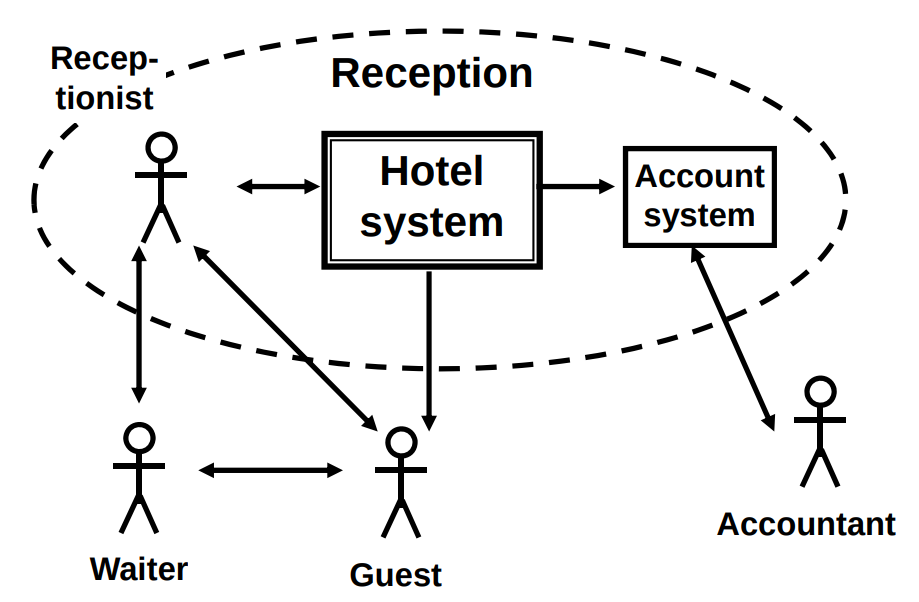
\includegraphics[width=\textwidth]{context-diagram.png}
  \caption{Reception domain in the Hotel system.}
  \label{figure:receptionDomainContextDiagram}
\end{figure}

You will now model the context diagram in Figure~\ref{figure:receptionDomainContextDiagram}. It should contain the elements: \textit{User, Domain, Product, System; interactsWith}

Transform this context diagram into a reqT model, this can be done using the REPL or the webeditor. Viewing \textit{interactsWith} as a doubly-linked arrow simplifies the context diagram model.

Finally, we'll use the reqT-REPL to produce an HTML document with a view of our context model. It is also possible to produce: graphs using GraphViz, Latex output, and Scala code.

\begin{framed}
\noindent A model have methods such as \texttt{toGraph}, \texttt{toLatex}, and \texttt{toHtml}.\\
\noindent We may produce an html document, given that a model is stored in $myModel$:
{
  \footnotesize\begin{verbatim}
  reqT> myModel.toHtml.save("myModel.html")
  \end{verbatim}
}
\noindent You will show your lab supervisor this HTML document (of the Context Diagram) --- also do this for the model in assignment 1 (\textit{QuackQuackGo}).

\noindent If you edit your model in the reqT-REPL you may want to save it to text (and version control it or view it in the reqT-webeditor)
{
    \footnotesize\begin{verbatim}
    reqT> myModel.toScala.save("myModel.scala")
    \end{verbatim}
}
\end{framed}
\end{enumerate}

%
% MANDATORY ASSIGNMENTS
%
\section{Model Assignments}\label{section:mandatoryAssignments}

In the following assignments you are going to be working with a system called DuSlang. DuSlang is a video streaming service with two types of users: video viewers, and video creators. DuSlang relies on advertisement revenue and utilizes an ad system called ReklamSinne - this delegates the ad handling to the third party service.

Here follows an incomplete model of the DuSlang requirements specification which you will complete and build upon - the source file is available on the course web page. As you may notice it follows the ReqBox structure you've been introduced to in the lectures. \textit{Note:} The Delivery section has been stripped away from this model view.

%
% MODEL START
%
\begin{framed}
\begin{lstlisting}
\end{lstlisting}
       \section*{context}
\begin{lstlisting}
\end{lstlisting}
       \subsection*{stakeholders}
\begin{lstlisting}
User videoCreator
  Spec ______
User videoViewer
  Spec ______
\end{lstlisting}
       \subsection*{product}
\begin{lstlisting}
______
\end{lstlisting}
       \subsection*{systems}
\begin{lstlisting}
System ReklamSinne
  Spec ______
\end{lstlisting}
       \subsection*{interfaces}
\begin{lstlisting}
\end{lstlisting}
       \section*{intentions}
\begin{lstlisting}
\end{lstlisting}
       \subsection*{goals}
\begin{lstlisting}
Goal advertisementDistribution
  Spec DuSlang shall ensure that advertisements are received by (shown to) the videoCreator and videoViewer
Goal freeVideoDistribution
  Spec DuSlang shall ensure that videoCreators may distribute their media freely (as in a zero cost upload)

\end{lstlisting}
       \subsubsection*{priorities}
\begin{lstlisting}
\end{lstlisting}
       \subsection*{risks}
\begin{lstlisting}
\end{lstlisting}
       \subsection*{commitments}
\begin{lstlisting}
\end{lstlisting}
       \section*{requirements}
\begin{lstlisting}
\end{lstlisting}
       \subsection*{functions}
\begin{lstlisting}
Feature subscriptions
  Why To enable a videoViewer to follow their favorite videoCreator
  Spec The videoViewer should be able to get an overview of the latest videos from their favorite videoCreators
Feature favorites
  Why So that a videoViewer may easily access an older video they watched
  Spec ______
  Example ______
Feature history
  Why ______
  Spec ______
Feature videoViews
  Why ______
  Spec Views shall be recorded when a video has been viewed for more than 10 seconds - or when the full length has been viewed
Feature videoLikes
  Why ______
  Spec Record the amount of like votes a video has received from its viewers
Feature videoDislikes
  Why ______
  Spec Record the amount of dislike votes a video has received from its viewers
Feature recommendedVideos
  Spec ______
Feature uploadVideo
  Spec ______
Feature playVideo
  Spec ______
Feature playAdvertisement
  Why ______
  Spec An advertisement should be played before playing the video to be viewed by the user
Feature useAdvertisement
  Why So that it is possible to make use of the advertised content
  Spec The videoViewer should be able to access the contents of the viewed advertisements
\end{lstlisting}
       \subsection*{data}
\begin{lstlisting}
______
\end{lstlisting}
       \subsection*{qualities}
\begin{lstlisting}
\end{lstlisting}
       \subsection*{tests}
\begin{lstlisting}
\end{lstlisting}
\end{framed}
%
% MODEL END
%

\subsubsection*{1. Introducing a context}
The section \textit{product} in the \textit{context} section should contain a context diagram of the DuSlang system. Fill in the product section of the DuSlang model. This is how a modeled context diagram might look given a hotel system, followed by the context diagram in figure~\ref{figure:hotelSystem}:

{\footnotesize\begin{verbatim}
Model(
  Section("context") has (
    Section("product") has (
      Product("hotelApp") interactsWith (
        User("receptionist"), 
        User("guest"), 
        System("telephony"), 
        System("accounting")))))
\end{verbatim}}

\begin{figure}[H]
  \centering
  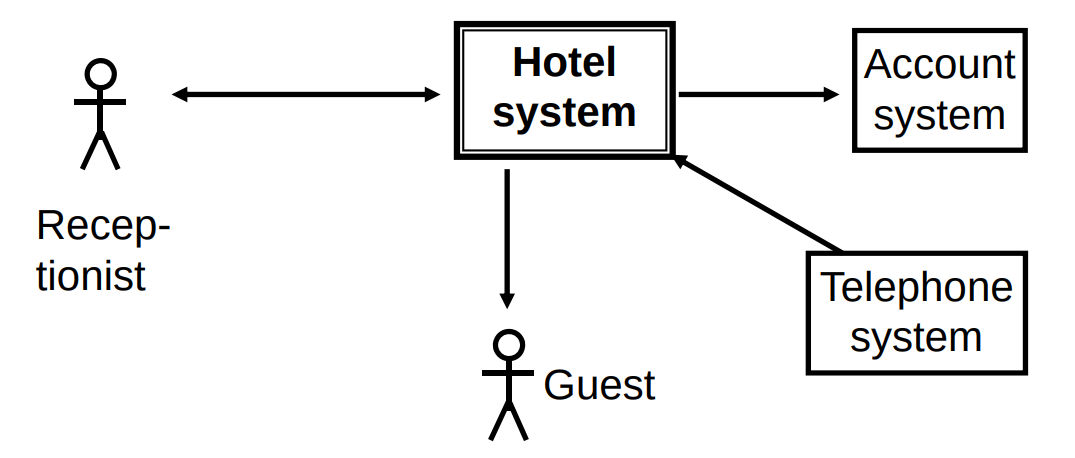
\includegraphics[width=\textwidth]{context-diagram-hotel-system.png}
  \caption{Context diagram of the hotel system.}
  \label{figure:hotelSystem}
\end{figure}


\subsubsection*{2. Finalizing features}
Now we'll move on to the \textit{functions} section, as seen in the model the functions section are missing some field values. You need to fill in these fields and you may use the informal system description of DuSlang below - from which the features have been elicited.

\begin{framed}
\subsection*{DuSlang system description}
One of the goals of the service is to supply everyone with a free medium of video distribution. This should be made possible by distributing advertisements received from a third party supplier - and this revenue may be re-invested to improve the service.

From a user perspective the service should provide an ease of use. This implies easily accessing their favorite videos or videos they have previously viewed. As noted in similar video services, users like to express their feelings towards a video - showing whether they liked it or not. It has been noted from similar video services that comment sections provide a very toxic (as in the informal sense) environment, thus DuSlang will not provide this feature.

Based on what kind of videos the video viewers are consuming we want to recommend them similar video material, therefore every viewer shall get individual video recommendations.

Video viewers often want to watch popular videos, to measure popularity (or lack thereof) video views, likes, and dislikes shall be measured. This is also interesting data for the video creator to verify whether they are producing good media content or not.

The user is also a big driver in providing the video content for our service. Allowing the user to freely distribute their video media will supply the viewers of the service directly. It is also possible for entertainment companies to distribute their video media on the platform - both as a means of advertising and providing it for their followers.

\end{framed}

\subsubsection*{3. Introducing a new goal}
Introduce a new goal for the video service. Make sure that you elicit the features necessary for fulfilling this goal.

% Let the student produce data or quality requirements?
% E.g. Specify the Data Requirements in the scope of a video - what data do we need to store? You should be able to elicit these requirements from the Features section.

\subsubsection*{4. Specifying data requirements}
Some of the features in our model, such as videoViews and videoLikes, will need to store data in our system. DuSlang shall store the following data on a per video basis: views, likes, and dislikes. Model this in the \textit{data} section.

\subsubsection*{5. Introducing relationships}
Given our goals, what features do we require? For each goal, link the required feature to the goal using relations. It is okay to reference an entity from another scope in the model as entity identifiers are to be seen as unique and global. This notion of cross-referencing is very graph-like.

\subsubsection*{Verification checkpoint}
Verify the results of this section with the lab instructor and continue with Section~\ref{section:extraAssignments}.

%
% EXTRA ASSIGNMENTS
%
\section{Metamodel Assignments}\label{section:extraAssignments}
In the following section we'll describe the metamodel, by this we mean the model that describes the reqT model that you used in the previous section (the model of a model, thereby the \textit{meta} prefix).

These assignments are focused on teaching fundamental principles of the REPL and metamodel. To get started you may follow these steps:

\textit{Note:} You may skip this if you already have a copy of the reqT.jar

\begin{framed}
\noindent Download the reqT jar
{\small\begin{verbatim}
curl -O http://reqt.org/reqT.jar
\end{verbatim}}
\noindent And launch the REPL
{\small\begin{verbatim}
java -jar reqT.jar
\end{verbatim}}
\end{framed}

\subsection{Create and update models using the reqT console}

\begin{framed}\noindent
Type in the following lines in the reqT console after the \verb+reqT>+ prompt. Press enter after each line. The \verb?+? operator is used to add elements to a model, and the  \verb?++? operator is used to append one model to another.

{\small\begin{verbatim}
reqT> val m1 = Model(Req("a") has Spec("sss"))

reqT> val m2 = m1 + (Req("b") has Prio(2))

reqT> val m3 = Model(Stakeholder("x") requires Req("a"))

reqT> ((m3 + Stakeholder("y")) ++ m2).size
\end{verbatim}}


\noindent What is the integer value result of the last evaluation above? Why?
\newline 
\newline
\newline \underline{\hspace{10cm}}

\vspace{7mm}
\noindent Continue to type in the following lines in the reqT console after the \verb+reqT>+ prompt. Press enter after each line. The \verb+for+ keyword is used to make a for-loop. The \verb+yield+ keyword is used in a for-loop to construct a sequence of values, that are picked one by one by the reserved  \verb+<-+ operator.  The \verb+val+ keyword is used to declare a name that refers to an immutable value (a constant) and the \verb+var+ keyword is used to declare a name that refers to a mutable value (a variable). The \verb?-? operator is used to remove elements from a model. With the \verb+transform+ method you can make transformations of specific elements in a model. 


{\scriptsize\begin{verbatim}
reqT> var m4 = (for (i <- 1 to 10) yield Req("r"+i)).toModel

reqT> (1 to 10).map(i => Req("r"+i)).toModel //alternative to above

reqT> m4 = Model(Stakeholder("x") requires m4)

reqT> m4 = m4 - Req("r7")

reqT> m4 -=  Req("r3")

reqT> m4.pp   //pretty-print m4

reqT> m4 = m4.transform{case Req(id) => Feature(id) has Status(ELICITED)}
\end{verbatim}}
\end{framed}
\begin{framed}\noindent
What is the size of the m4 model after the above transform? Why?
\newline
\verb+m4.size+
\newline
\newline \underline{\hspace{10cm}}
\end{framed}

\subsection{Investigate the reqT metamodel}

A reqT model can be viewed as a vector of elements. Elements can be entities, attributes and relations. An entity has an id of type String. An attribute holds a value that can be of different types. A relation connects an entity via a link of a certain RelationType to a submodel that, in turn, can contain elements. A part of the reqT metamodel is shown in Figure~\ref{figure:metamodel}. 

Investigate what different entity types, attribute types and relation types that the reqT metamodel contains, using the evaluations in the reqT console below. 

\begin{framed}{\footnotesize\begin{verbatim}
reqT> reqT.metamodel.  // Press <TAB> after the dot

reqT> reqT.metamodel.ent // Press <TAB> after the t

reqT> reqT.metamodel.entityTypes

reqT> reqT.metamodel.entityTypes.size

reqT> reqT.meta.model.pp

reqT> reqT.meta.model.collect{case Meta(_) => 1}.sum
\end{verbatim}}
\noindent The collect method gathers selected parts of a model into a vector. In the last evaluation above we collected the integer 1 for each occurrence of a Meta entity and sum all ones.
\newline\newline 
\noindent
How many different entity types, attribute types and relation types are there respectively in the reqT metamodel? 
\newline
\newline \underline{\hspace{10cm}}
\newline\newline
How many entity concepts of type \verb+Meta+  are there in the reqT metamodel (as calculated by the last evaluation above)? 
\newline
\newline \underline{\hspace{10cm}}
\end{framed}

The meta model elements can be used in many different ways. There are no restrictions on how to combine the elements, except for these three basic rules:
\begin{enumerate}[nolistsep]
\item {\bf Attribute identity}. A model or submodel can only contain at most {\it one} attribute of a specific type at its top level. However, the same type of attribute can co-exist if they reside in different submodels of the same model. 
\item {\bf Entity-Link identity}. A model or a submodel can only contain at most {\it one} entity with a certain id and a certain relation link at its top level. If you add an entity with the same id and the same relation link at the top level of a model or submodel, it will merge the elements of each submodel, and if the above rule applies then the last same-typed attribute will be overwrite the former. 
\item {\bf Leaf entity has empty submodel}. The \verb+has+-relation is special, as a leaf entity that has no relations to any subelements is equivalent to an entity with a has-relation to an empty submodel. 
\end{enumerate}

\begin{framed}\noindent
Try the subsequent statements in the reqT console, where \verb+Prio+ is an attribute type and \verb+Req+ is an entity type and \verb+has+ and \verb+requires+ are relation types. Make sure you can explain the evaluation results in relation to the rules above. Write the number of the rule(s) (1 -- 3) that is/are in effect besides each evaluation. 

{\scriptsize \begin{verbatim}
reqT> Model(Prio(1), Prio(2))

reqT> Model(Req("x") has (Prio(1), Prio(2)))

reqT> Model(Req("x") has Prio(1), Req("y") has Prio(1))

reqT> val m6 = Model(Req("x") has (Req("sub1"), Prio(1), Prio(2))) 

reqT> m6 + (Req("x") has (Req("sub2"),Prio(3)))

reqT> Model(Req("x") has ())

reqT> Model(Req("x") has Prio(1), Req("y") requires Prio(1)) - Prio(1)
\end{verbatim}}
\end{framed}

\begin{framed}\noindent
Create a model with two stakeholders \verb+a+ and \verb+b+, both requiring the same two features \verb+x+ and \verb+y+. The stakeholders' features shall have different priorities: a thinks x is of higher priority than y, while b thinks the opposite. Declare a constant called \verb+prio+ that refers to the model. Write the reqT code that describes your model below and then test it in the reqT console.
\newline
\newline 
\vspace{3cm}

\end{framed}

When you create a reqT model, you actually create an immutable, tree-like data structure that consists of computational objects in the Java Virtual Machine (JVM) runtime environment. When you encode reqT models you are actually coding in the \href{http://en.wikipedia.org/wiki/Scala_\%28programming_language\%29} {Scala programming language} that compiles to JVM byte code. The reqT metamodel classes are actually Scala classes and the reqT language is embedded in Scala. The \verb+reqT.jar+ file includes the Scala compiler and the reqT console wraps the so called Scala Read-Evaluate-Print-Loop (REPL), which enables any Scala code snippet to be interactively compiled and run on a line-by-line basis at the reqT prompt. 
\subsection{Access elements in models using paths}

A model is represented using a recursive data structure where relation elements can include submodels, which in turn can include relation elements that include submodels. The recursive nature of the model data structure thus enables hierarchical, tree-like requirements models of arbitrary depths. The submodels and elements of submodels at different levels can be extracted using paths that are constructed using the \verb+/+ operator called {\it enter}. 

A {\it head} is a start of a relation that combines an entity with a relation type using dot notation, such as  
\verb+Feature("x").has+ and \verb+Stakeholder("b").requires+  

Paths begin with a sequence of {\it heads} separated by \verb+/+ and may end with either (1) a head, (2) an entity, (3) an attribute type or (4) an attribute. The \verb+has+ relation is special: in paths an entity without any relation type is interpreted as an entity with a \verb+has+ relation. 

\begin{framed}\noindent
Try these path examples in the reqT console: 
{\scriptsize \begin{verbatim}
reqT> val p1 = Stakeholder("a").requires/Feature("x").has/Prio(42)

reqT> p1.depth    //write down the depth: _______

reqT> val p2 = Stakeholder("b")/Feature("x")/Prio(21)

reqT> p2.init     //what does the init method on a Path do? _________________ 

reqT> val p3 = p2.init/Feature("sub")/Prio(9)

reqT> p3.toModel

reqT> var pm = Vector(p1,p2,p3).toModel

reqT> pm/Stakeholder("b").has

reqT> pm/Stakeholder("b")

reqT> pm/Stakeholder("a").requires/Feature("x")/Prio

reqT> pm = pm + Stakeholder("a").requires/Feature("x")/Prio(1)

reqT> pm.leafPaths

reqT> pm.leafPaths.map(_.depth).max   //write down the max depth: ______
\end{verbatim}}
\end{framed}
\begin{framed}\noindent
Create a random model using the commands below, and write down its max depth: \underline{\hspace{1cm}}
{\scriptsize \begin{verbatim}
reqT> val rm = rndModel(10)
 
reqT> rm.pp

reqT> rm.leafPaths.map(_.depth).max    // Write down the max depth: _____

reqT> rm.leafPaths.filter(_.depth == 2).head
\end{verbatim}}
\noindent Write down the path to the first attribute at level 2:\newline\newline
\underline{\hspace{11cm}}
\end{framed}
 
If a path ends with an attribute type, then it refers to the corresponding value that is boxed by that attribute in a model. If the attribute is not available when the path is applied to a model with the enter operator \verb+/+ then a default value is produced. 

If you want to check the absence or presence of a value you can use the \verb+get+ method on a model. The \verb+get+ method takes a path as parameter and returns a value boxed in an instance of the \verb+Option+ class; if there was, e.g.,  an integer value of 42 then the option class evaluates to \verb+Some(42)+ or if there is no value then it evaluates to \verb+None+. You can get the actual value of an \verb+Option+ instance by calling the get method.    

\begin{framed}\noindent
Try these attribute type path examples in the reqT console: 
{\scriptsize \begin{verbatim}
reqT> val m = Model(Req("x") has Prio(1), Req("y"))

reqT> m / Req("x") / Prio

reqT> m / Req("y") / Prio    //write the default Prio value here _____

reqT> m.get(Req("x")/Prio)

reqT> (m/Req("x")).get(Prio).get    //same effect as previous    

reqT> m / Req("x") get Prio    //equivalent to previous

reqT> m / Req("x") get Prio get    

reqT> m / Req("y") get Prio get    
\end{verbatim}}
\noindent What happens if you try to call the \verb+get+ method on a non-existing value, as in the previous evaluation?
\newline\newline\underline{\hspace{10cm}}
\end{framed}

\subsection{Load and save files from the reqT console}

You can load text files into strings and save strings into text files using commands similar to: 
\begin{verbatim}
val s = load("myFile.txt")
"my String".save("myStringFile.txt")
\end{verbatim}
The \verb+ls+ command prints a list of files in the working directory. The \verb+pwd+ command prints the path of the working directory. The \verb+mkdir("tmp")+ command creates a new directory called \verb+tmp+ and \verb+cd("tmp")+ changes working directory to the directory \verb+tmp+ if it exists.

You can also serialize a model to a binary file, which for large files may take less space compared to a text file and it may also be quicker to save and load a large binary model to and from disk compared to a text model. To serialize a binary model to disk, just call the save method on a model. To load a binary model from disk use the \verb+Model.load("filename.reqt")+ command. It is recommend to use the file suffix \verb+.reqt+ to show that it is a serialized binary file.

\begin{framed}\noindent
Check that you have the files from the lab preparations in your working directory and load your context model and convert it to a reqT model from a string using the following evaluations: 
{\scriptsize \begin{verbatim}
reqT> ls
context.scala
feat.txt

reqT> var m = load("context.scala").toModel

reqT> m = Model(Title("My Cool Product"), Section("Context") has m)

reqT> m.toString.save("context-v2.scala")
Saved string to file: C:/Users/bjornr/tmp/context-v2.scala

reqT> m.save("context.reqt")
Model serialized to file: context.reqt
\end{verbatim}}
\noindent Create a large random model using \verb+rndModel+ e.g. with these parameters: \newline{\scriptsize\verb+val r = rndModel(52,2)  //max 52 at top level and then max 26 etc.+} \newline and compare the binary model size on disk with the string model text file size, by checking the file sizes in your OS. If the text file is bigger then generate a larger model.  If the files get so big that it takes too much time, reduce the number of max elements at top level.\newline
\newline Number of elements in the model: {\footnotesize\verb+r.size+} \underline{\hspace{2cm}} 
\newline Size of binary file: {\footnotesize\verb+r.save("big.reqt")+}  \underline{\hspace{2cm}} 
\newline Size of text file: {\footnotesize\verb+r.toString.save("big.scala")+} \underline{\hspace{2cm}}
\end{framed}

\subsection{Edit requirements with the reqT ModelTreeEditor GUI}

The reqT ModelTreeEditor is a graphical user interface for navigating and updating reqT model. You start the editor with the \verb+edit+ command. You can start many ModelTreeEditor windows. 

You can also preload a ModelTreeEditor instance with a model, e.g. called \verb+m+, by simply passing it as a paramter to the edit command, e.g. \verb+edit(m)+. The ModelTreeEditor is shown in Figure~\ref{fig:gui}. You can start many ModelTreeEditor windows by repeating the edit command.

\begin{figure}[ht]
    \centering
    \includegraphics[width=0.95\textwidth]{gui.png}
    \caption{The reqT ModelTreeEditor graphical user interface.}
    \label{fig:gui}
\end{figure}

The reqT ModelTreeEditor gui has two parts:
\begin{itemize}
\item {\bf The Tree}. The Tree displays a tree view of a model, where each head node can be collapsed or expanded using the right and left arrows or by clicking on the handle by the left of the folder symbol. Model elements can be deleted using the forward DELETE key.
\item {\bf The Editor}. The Editor is aware of the reqT metamodel and Scala syntax and provides syntax coloring and code completion on model elements. Entities are of light blue color, relations are of red color and attributes are shown in green color. Reserved words of Scala are given a dark blue color.
\end{itemize}

The Tree and the Editor are two separate buffers, each having its own data. The Tree has its own reqT model converted to a javax.swing.JTree, while the content in the Editor can be any text (typically users have a textual representation of a reqT (sub)model undergoing  some update). 

By using the menu items in the Tree menu and the Editor menu you can transfer data from the Tree to the Editor and vice versa. You can also execute Scala code in the Editor by entering code in the Editor to the console for evaluation. The ModelTreeEditor has a number of convenient shortcuts to enable power users to quickly operate the Tree and Editor in concert.

\begin{framed}
Carry out these steps using the ModelTree Editor:
\begin{enumerate}
\item Investigate the {\bf Template} menu and enter a template model to the Editor and then transfer the model from the Editor to the Tree using <Ctrl+R>.
\item Select the {\bf Help} menu item {\it Shortcuts to Editor} and investigate the different shortcuts and locate where in the menus they are. 
\item Use the {\bf File} menu item {\it Load text file to Editor} to load your prepared model \verb+context.scala+ into the Editor.
\item Select the root tree node and replace the tree with the model in the Editor using the Ctrl+R shortcut.
\item Use the {\bf File} menu "Save As..." to save your context model into a new file \verb+context.reqt+ in binary format.
\item Make sure you have your context model in the editor. Double click on \verb+Product+ to select it. Then select the {\bf Metamodel} {\it -> Entity -> Context -> System} menu item to replace \verb+Product+ with \verb+System+
\item Use code completion with <Ctrl+SPACE> to change \verb+System+ to \verb+Component+ 
\end{enumerate}
\end{framed}

The Editor can toggle between two different textual representations of a model: (1) the normal scala code that we have been using so far, and (2) a simplified model language called {\it ''reqT textified''} that represents models without any parenthesis and quotes, while using indentation to represent levels of submodels. \footnote{A textified reqT model is analogous to the \href{http://en.wikipedia.org/wiki/Markdown}{markdown} representation of a html document.} The toggling is made using the <Ctrl+T> shortcut.


\begin{framed}
\noindent Carry out these steps using the ModelTree Editor:
\begin{enumerate}
\item Load your \verb+feat.txt+ file into the using the <Ctrl+L> shortcut.
\item Toggle between {\it textified} and scala representations by pressing <Ctrl+T> several times.
\item When you have toggled to a scala model representation of your features in the Editor, select the root tree node and press <Ctrl+R> to replace the tree with your feature model.
\item Click in the Editor pane to make sure that the Editor is in focus and press <Ctrl+A> to select all.
\item Replace the text in the editor by entering this code: {\scriptsize\begin{verbatim}
m =>
  m.transform{
    case Item(i) => Feature(i)
    case Text(i) => Gist(i)
  }
\end{verbatim}}



\item Select the {\it Replace selected node by applying function in editor} menu item in the {\bf Tree} menu, or use the <Ctrl+Alt+Shift+R> shortcut to apply the above function to the Tree model.


\item Enter this code in the Editor and then press <Ctrl+Alt+Shift+R>: {\scriptsize\begin{verbatim}
m =>
  println("Size: " + m.size)
  println("Depth:" + m.leafPaths.map(_.depth).max)
  println("Number of fetaures: " + 
    m.collect{case f: Feature => 1}.sum)
  m
\end{verbatim}}



\item Explain what the above function does. Check what is printed in the console and write down the numbers: 
\newline Size: \underline{\hspace{1cm}} Depth: \underline{\hspace{1cm}}  Number of features: \underline{\hspace{1cm}}

\item Select the root node of your tree and press <Ctrl+E> to edit the model,  <Ctrl+T> to toggle to a textified model, and then <Alt+S> to save the text in the file \verb+feat-v2.txt+


\item Enter \verb?1 + 41? in the editor and press <Alt+Enter>. What happens?
\end{enumerate}
\end{framed}

\subsection{Export/Import of models to inter-operate with other apps}

In order to inter-operate with other apps and services, reqT can export and import data in various formats. A general format of inter-operation is text, as you worked with in the previous section. With reqT, you can also inter-operate with html, tabular text, and other formats.

\begin{framed}
\noindent Carry out these steps using the ModelTreeEditor gui:
\begin{enumerate}[nolistsep,noitemsep]
\item Load the ''Model with sections'' in the {\it Templates} menu and press <Ctrl+R>.
\item Choose the Export -> ''HTML from tree ...'' menu and give a file name for the static site to be generated.
\item A browser window should appear on your desktop with the generated html file.
\item How are the different special elements Title, Section, and Text rendered in your browser? \newline\newline\underline{\hspace{10cm}}\newline
\item Inspect the html code generated in the index.html file. 
\end{enumerate}
\end{framed}

%%%% TODO PathTable Export and Import etc.

\begin{framed}
If you have \url{http://graphviz.org} installed on your machine, carry out these steps using the ModelTreeEditor gui:
\begin{enumerate}
\item Load your context.scala file into the Tree.
\item Choose the Export -> ''GraphViz .dot nested ...'' menu and give a file name for the generated graph.
\item A pdf reader window should appear on your desktop with the generated pdf file.
\item Compare with the ''GraphViz .dot flat ...'' export. \newline What is the difference between nested and flat graph export?
\newline\newline\underline{\hspace{10cm}}
\end{enumerate}
\end{framed}

\subsection{Investigate the Status attribute for tracking requirements evolution}

As requirements evolve, it is often interesting to keep track of how far we have come in the process from elicitation to release. To enable this, reqT has a \verb+Status+ attribute which boxes a status value that  represents states of a requirements state machine, where requirements can travel up and down a  ''release ladder''. In the subsequent tasks you will use the Editor to investigate the transitions between status values as requirements go up and down the ''ladder''.  

\begin{framed}
\noindent You can use the Editor to evaluate expressions and let the evaluation results be pasted into the Editor after the evaluation using the <Alt+Enter> shortcut. Enter the following code snippets and press <Alt+Enter> after each code snippet. When the Editor is in scope you can press <Ctrl+Z> to undo in several steps.
\begin{enumerate}[noitemsep,nolistsep]
\item Enter in editor: \verb+StatusValue.values+ and then press <Alt+Enter>.
\item Enter in editor: \verb+ELICITED.up+ and then press <Alt+Enter>. (You can use code completion to enter ELICITED without typing so much by entering E and the press <Ctrl+Space>.)
\item Enter in editor: \verb+ELICITED.down+ and then press <Alt+Enter>. Write down the status if you go down from \verb+ELICITED+ \underline{\hspace{3cm}}
\end{enumerate}
\end{framed}

\newpage %%%%%
\begin{framed}
\noindent Draw the state machine representing all reqT's built-in requirements status transitions by carrying out the steps below:
\begin{enumerate}
\item Use repeated evaluations with <Alt+Enter> in the Editor to check what happens if you call \verb+up+ or  \verb+down+ on all values in \verb+StatusValue.values+ respectively. Use <Ctrl+Space> to type faster. 
\item Draw below a \href{http://en.wikipedia.org/wiki/State_diagram}{state diagram} with all nodes \verb+ELICITED+, \verb+SPECIFIED+, etc., with two directed edges from each state labeled \verb+up+ and \verb+down+ respectively, showing all the transitions. \newline
\vspace{7cm}
\item Reflect upon what in a hypothetical project may be different paths of different features through the above diagram. Are there any transitions missing that you think might be needed? If so, why are they needed?
\item Type this code into the Editor and select the root node in the Tree and press <Ctrl+R>:{\scriptsize\begin{verbatim}
val up = StatusValue.values.map(v => 
  Label(v.toString) precedes Label(v.up.toString)).toModel
val down = StatusValue.values.map(v => 
  Label(v.toString) precedes Label(v.down.toString)).toModel
up ++ down
\end{verbatim}}
\item If you have \url{graphvis.org} installed on your machine you can now export the Tree to a flat GraphViz graph to see the state diagram.
\end{enumerate}
\end{framed}

\end{document}
